\chapter{Indledning}
Hormonet insulin er vigtigt til regulering af glukoseniveauet i blodet. Produktionen af insulin foregår i pancreas, nærmere bestemt i de langerhanske øer. Et fald i insulinproduktionen, grundet nedsat funktion af de langerhanske øer, kan føre til den livstruende sygdom \textit{diabetes mellitus (type 1)}. Prævalensen af diabetes mellitus er i Danmark på 320.545, hvor omkring 10 \% lider af type 1 diabetes \citep{diabetes}. På grund af den store udbredelse af diabetes er der stor interesse i forskning på området. Til forskningen bruges der ofte en stor mængde af langerhanske øer. 


\section{Baggrund}
For at undersøge sygdommen nærmere, samt øge forståelsen for de mekanismer, der styrer insulinreguleringen i kroppen udføres der videnskabelige forsøg med Langerhanske øer.

De øer der anvendes til videnskabelige forsøg stammer typisk fra mus eller rotter. Sortering- og isoleringsprocessen foregår ved tre faser \citep{per}, som vist i figur \ref{fig:sortproces}. 

\begin{figure}[H]
	\centering
	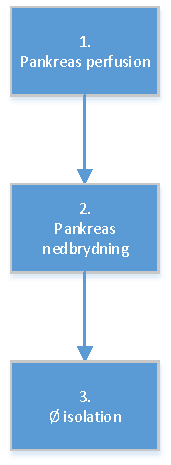
\includegraphics[width=0.2\textwidth]{billeder/sortering-crop.pdf}
	\caption{Faser i sorteringsprocessen}
	\label{fig:sortproces}
\end{figure}

I første fase, \textit{pankreas perfusion}, sprøjtes enzymet \textit{collagenase V} ind gennem galdegangene og derfra videre til  pankreas. Dette enzym starter en nedbrydning af vævet i pankreas. Herefter fjernes pankreas operativt. Enzymet collagenase har den egenskab, at det ikke nedbryder de langerhanske øer i samme grad som det omkringliggende eksokrine væv.

I anden fase, \textit{pankreas nedbrydning}, nedbrydes pankreas yderligere ved at inkubere pankreas ved 37° i 19 min. Ved denne temperatur er enzymet collagenase særligt aktivt og katalysere derfor nedbrydningen af pankreas. Herefter nedkøles vævet for at stoppe virkningen af collagenase.

% sker derfor relativt hurtigt.  den bliver skåret i mindre dele og pankreas placeres i en inkubator ved 37,5 grader. Dette gøres for at accelerere nedbrydningen af pankreas. Når pankreas er nedbrudt nedkøles vævet for, at stoppe virkningen af collagenase. 

I den sidste fase, \textit{ø isolation}, vaskes og rystes øerne først af tre omgange med en vaskebuffer i form af en saltvandsopløsning \citep{hbbs}. Dette gøres for at løsrive øerne fra hinanden inden isolering. Herefter er øerne klar til at blive isoleret fra det eksokrine væv. Der findes en række forskellige metoder til dette, hvor den mest udbredte metode foregår ved manuel isolering af øerne fra en petriskål vha. et mikroskop. Der bruges allerede automatiserede isoleringsmetoder bygget på forskellige teknikker, herunder gradientbaseret centrifugering. Fælles for de anvendte teknikker til isolering af øerne er, at der er stor risiko for skade på øerne. 

Denne manuelle metode har yderligere ulemper, idet den både er besværlig og tidskrævende. Herudover kan der være stor variation i kvaliteten af isoleringen, da der kan være forskel på den enkelte operatørs håndtering af øerne. 

Derfor ønskes der en automatiseret metode til isolering af langerhanske øer, med minimal risiko for skader på øerne. En automatiseret metode vil have følgende fordele \cite{pptintro}: 

\begin{itemize}
\item Øget sorteringshastighed for højere udbytte
\item Reducere variation i de isolerede øer
\item Reducere omkostningerne
\item Sikre bedre dokumentation
\item Forbedret arbejdsmiljø
\end{itemize} 

En automatiseret løsning vil potentielt åbne op for nye muligheder indenfor anvendelse af langerhanske øer. Der forskes bl.a. i transplantation af langerhanske øer, som et led i behandling af type 1 diabetes. Resultaterne af et af disse forskningsprojekter har bl.a. vist at 44 \% af modtagerne af denne type behandling var insulinuafhængige 3 år efter transplantation \citep{islettransplantation}. Til forskning er langerhanske øer bl.a. anvendt til at undersøge hvordan aminosyrer er glukoseafhængige \citep{aminosyre}. I forskningsforsøget er der brugt 6-10 mus, hvilket cirka har taget 6-10 timer at håndplukke (jvf. Per B. Jeppesen). Det er forskningsprojekter som dette, hvor en automatiseret løsning vil være relevant, da det vil skabe en mulighed for en større testgruppe og frigive ressourcer til andre formål i forsøget.

\newpage
På Medicinsk Endokrinologisk Afdeling (MEA), Aarhus Universitetshospital, er der tidligere arbejdet hen imod en automatiseret løsning til isolering af langerhanske øer. Den automatiseret løsning vil primært bidrage til forskningen, der foretages på afdelingen. Tidligere blev der udviklet en prototype til automatiseret ø-isolation, der fungerede ved hjælp af kameradetektion. Ved detektion sugede en pipette den detekterede ø op fra en petriskål. Pipetten blev styret i X,Y og Z retning vha. en mekanisk robotarm. Se figur \ref{fig:Tidliger prototype} for en illustration af den gamle prototype. \footnote{Kilde: Søren Gregersen}

\begin{figure}[H]
	\centering
	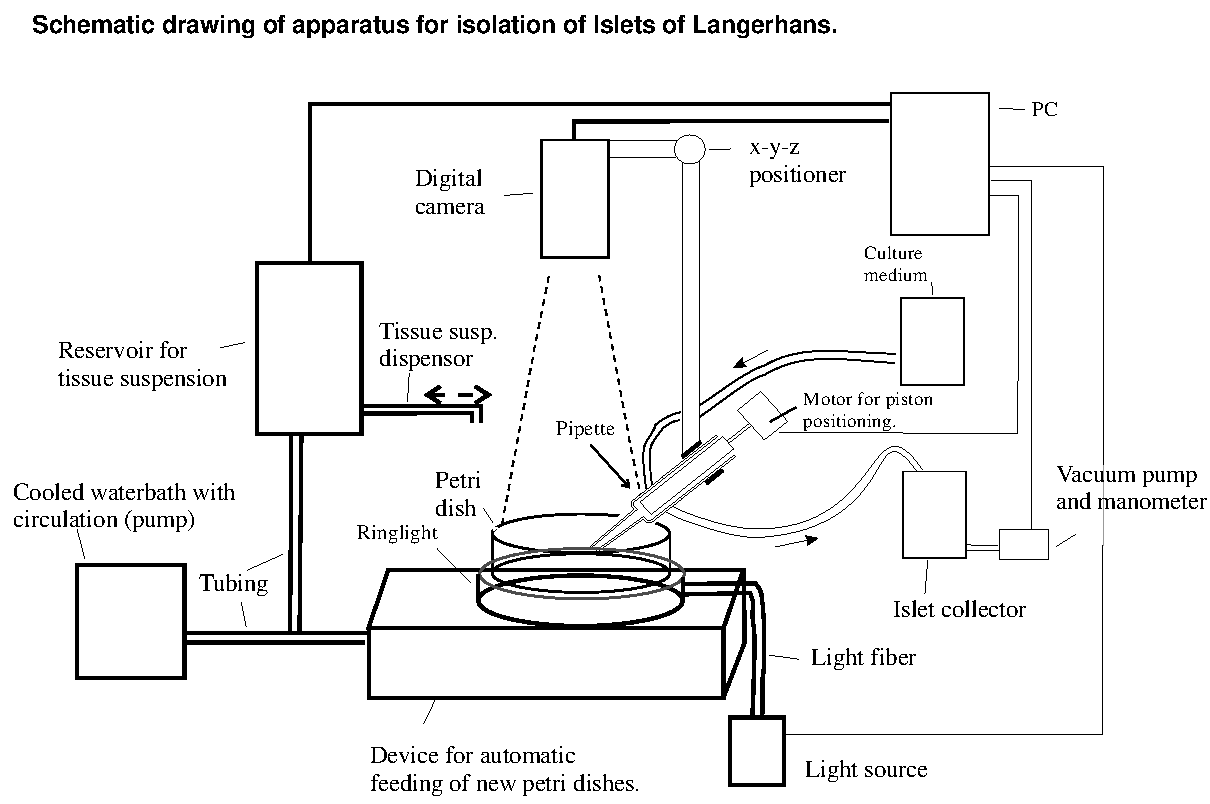
\includegraphics[width=1\textwidth]{billeder/hovedrapport/glprototype.pdf}
	\caption{Tidligere prototype}
	\label{fig:Tidliger prototype}
\end{figure}


 Prototypen var dog ikke præcis nok, primært pga. bevægelse i væsken, og projektet blev derfor stoppet.
 

%\textbf{Noter:}
%
%kilder om transplantation af øer
%
%
% 
% 
% find videnskabelige artikler der bekræfter at denne metode med at skyde langerhanske øer ind i sukkersyge mus/rotter virker og det er derfor dette projekt er mega relevant og pisse godt
% 
% derfor
% 
% - videnskabelig artikel over sorteringsprocessen
% 
% - videnskabelig artikel over at metoden virker, evt. hvorfor den ikke er mere brugt(sorteringsprocessen er for langsommelig)




\section{Problemformulering}

Målet med dette projekt er, i samarbejde med Medicinsk Endokrinologisk Afdeling, at udvikle et \textit{Proof of Concept} system til isolering af langerhanske øer. Systemet bygger videre på de erfaringer der blev opnået ved den tidligere prototype. Metoden til isoleringen baseres fortsat på kameradetektion, mens den mekaniske isolering i stedet erstattes med et ventilsystem. Det udviklede system skal altså kunne detektere langerhanske øer vha. billedprocessering for herefter at isolere øerne fra resten af opløsningen med en ventil. 

Herudover skal en cost-benefit analyse være med til, at belyse hvilke økonomiske og kvalitative fordele det udviklede system kan have, sammenlignet med den anvendte manuelle metode.

\section{Afgrænsning}
Til at afgrænse projektet anvendes \textbf{M}o\textbf{SC}o\textbf{W} modellen, som beskriver hvilke dele projektet skal (\textbf{M}ust), bør (\textbf{S}houd), kan (\textbf{C}ould og ikke (\textbf{W}ont) indeholde. MoSCoW modellen (figur: \ref{fig:moscow}) viser hvordan de enkelte krav og dele af projektet er prioriteret. 
Redegørelse og begrundelser for valg/fravalg
Moscow

\begin{figure}[H]
	\centering
	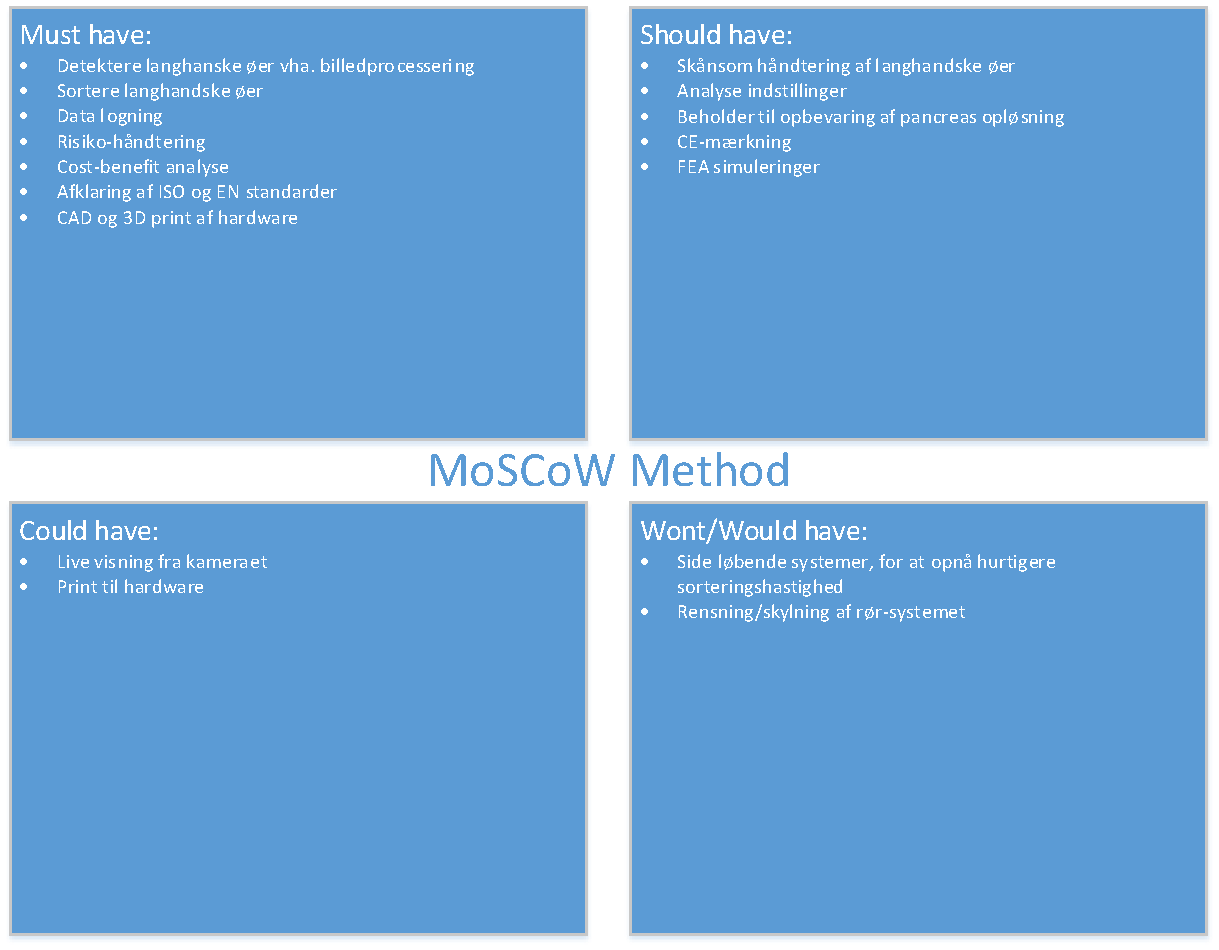
\includegraphics[width=1\textwidth]{billeder/MoSCoW-crop.pdf}
	\caption{MoSCoW}
	\label{fig:moscow}
\end{figure}

De krav systemet skal opfylde er bl.a. at kunne detektere langerhanske øer vha. billedprocessering, samt sortere øerne ved detektion. Herudover skal systemet kunne gemme data omkring de sorterede øer herunder størrelse og cirkularitet. Projektet består desuden af en cost-benefit analyse der beskriver hvilke fordele og ulemper det automatiserede system vil have. 

Et af de vigtigere krav der er nedprioteriet i projektet er skånsom håndtering af langerhanske øer. Denne del vil kræve en validering af den udviklede prototype igennem funktionstest af de isolerede langerhanske øer. Referencer til dette?

Dette projekt vil derfor i højere grad fokusere på en verificering af den udviklede prototype i form af en accepttest, som tester de funktionelle og ikke funktionelle krav.
